\chapter{Precision-Oriented Query Facet Extraction}
\label{ch:precision}
\todo{Why not do this earlier}
\section{Introduction}
\label{sec:precision-intro}
While the query facet extraction approach presented in Chapter~\ref{ch:facet} and intrinsic evaluation in Chapter~\ref{ch:intrinsiceval}, provide a promising direction for solving the open-domain facet generation problem, it neglects the precision-oriented perspective of the task, which we believe is important in practical use. As in many precision-oriented information retrieval tasks, we believe users are likely to care more about ``facet precision'' than ``facet recall''. That is, users may care more about the correctness of presented facets (\eg, are the terms in the airline facet indeed about airlines, and are the airline terms grouped together in a same facet) than the completeness of facets (\eg, are all possible facets for that query presented, and are all possible airline terms included the results?). In other words, mistakes of presenting wrong terms in a facet, or grouping terms incorrectly are more severe than omitting some facets or terms in facets. The work presented in Chapter~\ref{ch:facet} 
and Chapter~\ref{ch:intrinsiceval} does not consider 
this precision-oriented factor when designing query facet extraction models or evaluating 
extraction results. Therefore, it is unclear if these models can adapt to such scenarios.

In this chapter, we study query facet extraction under the precision-oriented scenario, and improve extraction performance under those scenarios from two perspectives.

First, we find the learning objective used in our query faceting models are not ideal for the task especially under the precision-oriented scenario. The proposed model is trained by maximum likelihood estimation on labeled training data. However, likelihood can be loosely related to the performance measure under the precision-oriented scenario. In this chapter, we propose to directly maximize the performance measure \PRF instead of likelihood during training using an empirical utility maximization (\EUM) approach. However, exact optimization on the performance measure is difficult due to the non-continuous and non-differentiable nature of information retrieval measures. We address this problem by approximating the performance measure using its expectation. We show that this empirical utility maximization approach significantly improves over previous approaches under precision-oriented scenarios, suggesting utility is a better learning objective than likelihood, and our expectation-based 
approximation is effective.  

Second, we improve extraction performance by a selective method that shows facets for good performing queries and avoids poor performing ones. We find that extraction performance varies for different queries -- some queries are naturally more difficult than others for extracting query facets. In the precision-oriented scenario, it may be more desirable to avoid showing facets for those poor performing queries and leave the users with a clean keyword-search interface. A key problem, however, is how to predict the extraction performance. To solve this problem, we propose a simple and effective score based on the expectation of the performance measure. We find the score has a strong correlation with the performance measure, and when used in the selective method, it can significantly improve the average performance with fair coverage over the whole query set.

The rest of this chapter is organized as follows. In Section~\ref{sec:precision-related}, we briefly review related work. In Section~\ref{sec:precision-measure}, we revisit the \PRF measures used in the intrinsic evaluation (Chapter~\ref{ch:intrinsiceval}) in order to help develop our empirical utility maximization approach in Section~\ref{sec:precision-eum}, and our selective method for query faceting in Section~\ref{sec:precision-selective}. We carry out experiments in Section~\ref{sec:precision-experiment}.
\section{Related Work}
\label{sec:precision-related}
\subsection{Directly Optimizing Performance Measures}
Lots of previous work has proposed to directly optimize performance measures in learning for various information retrieval tasks, including ranking~\cite{metzler2005direct,xu2008directly,xu2007adarank,cossock2006subset,quoc2007learning,de2007combined} and classification~\cite{musicant2003optimizing,joachims2005support,jansche2005maximum}. While higher performance is expected by doing so, it is usually difficult due to the non-continuous and non-differentiable nature of information retrieval measures. From the perspective of the loss function optimization, existing solutions fall into three categories~\cite{xu2008directly}. First, one can minimize the upper bounds of the basic loss function defined on the performance measures~\cite{xu2007adarank,joachims2005support,yue2007support}. Second, one can approximate the the performance measures with functions that are easy to handle~\cite{jansche2005maximum,cossock2006subset}. Our work belongs to this category; it approximates the performance measure using a 
continuous function based on 
its expectation. Third, one can use specially designed technologies for optimizing the non-smooth performance measures~\cite{quoc2007learning,de2007combined}. 

More related to our problem, Jansche proposed to train a logistic regression model by directly optimizing F-measures~\cite{jansche2005maximum}. The work approximated integer quantities in F-measures based on their probabilities, and thus made the optimization target continuous and differentiable. Then it trained the logistic regression model by optimizing the approximated F-measures on the training data. The method is also referred to as empirical utility maximization (or empirical risk minimization)~\cite{ye2012optimizing}, which maximizes the expected utility (or performance) by its average utility on the training data as an approximation. The model and measure we study in this paper (see Section~\ref{sec:facet-gm} and \ref{sec:ie-metrics}) is similar to Jansche's work, and we use similar approximation strategy in order to perform direct optimization on the performance measure.

\subsection{Performance Prediction and Selective Methods}
Previous work on performance prediction in information retrieval primarily focused on the core ranking problem. Many predictors/scores have been introduced for predicting retrieval performance, such as clarity score~\cite{cronen2002predicting}, average IDF~\cite{tomlinson2004robust} and robustness score~\cite{zhou2006ranking}. Learning methods, such as regression models, have also been used to combine different factors for predicting retrieval performance~\cite{kwok2004trec,balasubramanian2010predicting,yom2005learning}. 

One application of retrieval performance prediction is to allow the systems to invoke alternative retrieval strategies for different queries according to their performance. For example, \citet{yom2005learning} and \citet{amati2004query} showed that retrieval performance prediction can be used to improve the effectiveness of a search engine, by performing selective
automatic query expansion for ``easy'' queries only. Our selective method for query facet extraction is similar to these methods in spirit -- we want to selectively apply query facet extraction for ``easy'' queries only. However, to the best of our knowledge, no existing work has studied performance prediction for query facet extraction.

\section{\PRF Measure}
\label{sec:precision-measure}
Our empirical utility maximization approach, selective method for query faceting and evaluations for them are all based on the \PRF measure that was introduced in Chapter~\ref{ch:intrinsiceval}. In this section, we revisit this measure, and reformulate it in a way that will make the development for the utility maximization approach and the selective method easier. Recall that the \PRF measure combines term precision, term recall, and term clustering performance. We will describe the different aspects in the following sections.

\subsection{Notation}
We continue to use notation defined in Section~\ref{sec:facet-formulation} and Section~\ref{sec:evalmetrics}. The term label $y_i$ indicates whether the list item $t_i$ is indeed a facet term. The pair label $z_{i,j}$ indicates whether the list item $t_i$ and $t_j$ are in the same query facet. To help describe the measure, we use superscript ``$*$'' to distinguish ground truth labels from system predicted labels. For example, $y_i^*$ is a ground truth term label, while $y_i$ is a term label predicted by the system. Similarly, $z_{i,j}^*$ is a ground truth pair label, while $z_{i,j}$ is a predicted pair label. 
%$T_\mathcal{F}^*$ is a set composed of all the terms in the ground truth facets, while $T_\mathcal{F}$ is consisted by all terms in the system extracted facets.

\subsection{Term Precision and Recall}
In \PRF, the classification performance is measured by term precision (\ie, precision of the selected candidate terms being facet terms) and term recall (\ie, recall of facet terms).  They can be formulated as below, where subscript ``$c$'', ``$s$'', ``$g$'' stands for ``correct'', ``system'', ``ground truth'' respectively.
\begin{itemize}
 \item Term precision: $T\!P = \frac{T_c}{T_s}$, where $T_c$ is the number of correct facet term selected, $T_s$ is the number of terms select by the system. 
 \item Term recall: $T\!R = \frac{T_c}{T_g}$, where $T_c$ is as defined above, $T_g$ is the number of facet terms in the ground truth.
 \item Term F1: $T\!F=\frac{2T_c}{T_s+T_g}$ is the F1 combination (or harmonic mean) of $T\!P$ and $T\!R$.
\end{itemize}

The Quantities $T_c$, $T_s$, $T_g$ can be more precisely defined using term labels $y_i$ and $y_i^{*}$ as
\begin{equation}
\label{eq:qterm}
 T_c=\sum_i{y_iy_i^{*}}, \;\; T_s=\sum_i{y_i}, \;\; T_g=\sum_i{y_i^{*}}.
\end{equation}

\subsection{Term clustering}
%Our re-examination finds that the term clustering measure used in \PRF could double-count term recall factor. The problem stems from  that the terms being clustered by the model can be different from the terms clustered in the ground truth, \ie, $T_\mathcal{F}\neq T_\mathcal{F}^{*}$. $T_\mathcal{F}$ may include wrong terms or miss correct facet terms. Standard clustering measures typically cannot handle these cases properly. Therefore, Kong and Allan~\cite{kong2013extracting} adjust the extracted facets $\mathcal{F}$ as if only facet terms in $T_\mathcal{F}^{*}$ were clustered by the system. This is done by removing incorrect terms ($t\in T_\mathcal{F}-T_\mathcal{F}^*$) from $\mathcal{F}$, and adding each missing facet terms ($t^{*}\in T_\mathcal{F}^*-T_\mathcal{F}$) as singletons. They claimed that by this adjusting, term clustering performance does not take into account the effectiveness of finding facet terms, but we find it actually incorporates term recall factor. Analytically, we can see that when a 
system fails to find a facet term, by assuming it being a singleton, the clustering performance will be hurt (unless the facet term is a singleton in the ground truth). Empirically, we find systems return large sized facets when tuned on term clustering performance based on the adjusting. For example, on average, QFI returns 509.8 terms per query, while there is only 81.2 facet terms per query in the ground truth. Therefore by combining term precision, recall and clustering performance, $P\!R\!F_{\alpha,\beta}$ actually double-counts the term recall factor by this adjusting when measuring clustering performance. 

In \PRF, term clustering performance is measured by pair-counting F1 measure after clustering adjusting (Section~\ref{sec:intrinsic-pmeasures}). Here the pair-counting F1 measure treats term clustering as classification on whether each pair of terms is in the same facet, and then combines pair precision and recall using the F1 measure. Pair precision and recall can be formulated as below. (The subscripts carry the same meaning as in term precision and recall.)
\begin{itemize}
 \item pair precision: $P\!P = \frac{P_c}{P_s}$, where $P_c$ is the number of term pairs the model clustered together that are indeed in the same facet in the ground truth, $P_s$ is the number of term pairs the model clustered together. 
 \item pair recall: $P\!R = \frac{P_c}{P_g}$, where $P_c$ is as defined above, $T_g$ is the number of term pairs clustered together in the ground truth.
 \item pair F1: $P\!F=\frac{2P_c}{P_s+P_g}$ is the F1 combination (or the harmonic mean) of $P\!P$ and $P\!R$.
\end{itemize}

The quantities $P_c$, $P_s$, $P_g$ can be more precisely defined using term labels $y_i$,$y_i^{*}$ and pair labels $z_{i,j}$, $z_{i,j}^{*}$ as
\begin{equation}
\label{eq:qpair}
 P_c=\sum_{i,j}{z_{i,j}z_{i,j}^{*}}, \; P_s=\sum_{i,j}{z_{i,j}}y_i^*y_j^*, \; P_g=\sum_{i,j}{z_{i,j}^*}y_iy_j,
\end{equation}
where term labels $y_i$,$y_i^{*}$ are used to perform the cluster adjusting (Section~\ref{sec:intrinsic-pmeasures}), after which only the clustering performance on the correctly selected facet terms are evaluated.

\subsection{Combining term precision, recall and clustering}
The quality of query facet extraction is intrinsically multi-faceted. Different applications or scenarios might have different emphases among the term precision, recall and clustering. To address this issue, $P\!R\!F_{\alpha,\beta}$ combines the three factors together, using weighted harmonic mean. We repeat its formulation below,
\begin{equation}
\label{eq:prf2}
 P\!R\!F_{\alpha,\beta}(T\!P, T\!R, P\!F) = \frac{(\alpha^2 + \beta^2 + 1)}{\frac{\alpha^2}{T\!P} + \frac{\beta^2}{T\!R} + \frac{1}{P\!F}}.
\end{equation}
Note that $\alpha,\beta \in [0,+\infty)$ are used to control the weight between the three factors. $\alpha$ and $\beta$ can be interpreted as the importance of $T\!P$ and $T\!R$ compared to $P\!F$ respectively (Section~\ref{sec:evalmetricsall}).

To evaluate query facet extraction under the precision-oriented scenario, we can set a high $\alpha$ and/or low $\beta$. For example, we can set $\alpha\!=\!2,\beta\!=\!1$ to evaluate the case where $T\!P$ is twice as important as $T\!R$ and $P\!F$. Perhaps more reasonably, we can only down-weight the recall factor, by setting $\alpha\!=\!1,\beta\!=\!1/3$ to evaluate the case where $T\!P$ and $P\!F$ are three times as important as $T\!R$.

To help develop our empirical utility maximization approach, we rewrite $P\!R\!F_{\alpha,\beta}$ as a function of term and pair quantities $T_c,T_s,T_g,P_c,P_s,P_g$ as
\begin{equation}
\label{eq:prfc}
 P\!R\!F_{\alpha,\beta}(T_c,T_s,T_g,P_c,P_s,P_g) =\frac{2(\alpha^2 + \beta^2 + 1)T_cT_p}{2\alpha^2T_sP_c+2\beta^2T_gP_c+T_cP_s+T_cP_g}.
\end{equation}
It is easy to see $P\!R\!F_{\alpha,\beta}$ can be also rewritten as a function of predicted labels and ground truth labels as $P\!R\!F_{\alpha,\beta}(Y,Z,Y^{*},Z^{*})$ by substituting term and pair quantities using Equation~\ref{eq:qterm} and~\ref{eq:qpair}.

%\cmt{add comments for weighted version of PRF and other measures}

\section{Empirical Utility Maximization}
\label{sec:precision-eum}
\todo{present all derived equations}
In this section, we describe our empirical utility maximization (\EUM) approach that directly optimizes \PRF for training the query faceting (\QF) model (described in Section~\ref{sec:facet-gm}). 

The \QF model can be viewed as a model which takes in candidate terms and term pairs and predicts their labels, $(Y, Z)=h(T_\mathcal{L},P_\mathcal{L};\lambda,\mu)$. The parameters $\lambda,\mu$ are trained by maximizing the conditional likelihood of the labels, $l(\lambda,\mu)$ as defined in Equation~\ref{eq:ll}. One problem with the maximum likelihood estimation is that the likelihood target can be loosely related to performance measure $P\!R\!F_{\alpha,\beta}$, especially in the precision-oriented scenario, where term recall is less important than other factors (as we will show in Section~\ref{sec:precision-experiment}).

Therefore, we propose an alternative way of training the model $h(T_\mathcal{F},P_\mathcal{F})$ by directly optimizing the $P\!R\!F_{\alpha,\beta}$ measure. Our goal is to maximize the expected utility (or performance),
\begin{equation}
 E_\mathcal{P}\big[P\!R\!F_{\alpha,\beta}(h(T_\mathcal{L},P_\mathcal{L}),Y^*,Z^*)\big],
\end{equation}
where $\mathcal{P}$ is the underlying and unknown distribution of our data $(T_\mathcal{L},P_\mathcal{L},Y^*,Z^*)$. In order to train the model, empirical utility maximization (or equivalently empirical risk minimization) is usually used, which tries to maximizes the above utility objective function over empirical data,  $\mathcal{D}=\{T_{\mathcal{L}}^{(i)},P_{\mathcal{L}}^{(i)},Y^{*(i)},Z^{*(i)}|i=1...n\}$. The empirical utility is given below, 

\begin{equation}
\begin{split}
 U(\lambda,\mu) &= E_\mathcal{D}\big[P\!R\!F_{\alpha,\beta}(h(T_\mathcal{L},P_\mathcal{L}),Y^*,Z^*)\big] \\
 &=\frac{1}{n}\sum_{i=1}^{n}P\!R\!F_{\alpha,\beta}(T_c^{(i)},T_s^{(i)},T_g^{(i)},P_c^{(i)},P_s^{(i)},P_g^{(i)}),
\end{split}
\end{equation}
where we use the uniform distribution over empirical data to replace the unknown distribution, and replace the $P\!R\!F_{\alpha,\beta}$ term with $P\!R\!F_{\alpha,\beta}$ calculation based on term and pair quantities $P\!R\!F_{\alpha,\beta}(T_c,T_s,T_g,P_c,P_s,P_g)$ as defined in Equation~\ref{eq:prfc}. 

Our goal now is to find $(\lambda,\mu)=\argmax_{\lambda,\mu}{U(\lambda,\mu)}$. Unfortunately, this objective is difficult to optimize. The basic quantities involved are integers, and the optimization objective is a piecewise-constant function of the parameters $\lambda$, $\mu$. The non-smoothness is because the dependent variable $y_i$ and $z_{i,j}$ take only discrete values $\{0,1\}$. For example, $U(\lambda,\mu)$ contains integer quantity $T_c=\sum_i{y_iy_i^{*}}$ that counts the correct facet terms labeled. According to QFI (see Section~\ref{sec:facet-infer}), $y_i$ is predicted as either 1 or 0 by thresholding its term probability $P(y_i=1|t_i)$ as:
\begin{equation}
 y_i = 1\{P(y_i=1|t_i)>w_{min}\},
\end{equation}
where $P(y_i=1|t_i)=\frac{1}{1+\exp\{-\sum_k{\lambda_k f_k(t_i)}\}}$ (defined in Equation~\ref{eq:y}) involves parameter $\lambda$. Thus, $U(\lambda,\mu)$ is a piecewise-constant function of $\lambda$. The same applies for $\mu$ as well.

In generally, we can approximate discrete variables by their expectation to obtain a smooth objective function~\cite{jansche2005maximum}. In our case, by assuming independence between all the labels, $y_i$ can be approximated by its expectation as, 
\begin{equation}
 \widetilde{y}_i = E[y_i]= P(y_i\!=\!1|t_i)= \sigma(\lambda^T f(t_i)),
\end{equation}
where we use $\sigma(x)=\frac{1}{1+\exp\{-x\}}$ to denote the logistic function used in Equation~\ref{eq:y}, and use vector-representation for $\lambda$ and feature $f(t_i)$ for convenience. Similarly, we approximate $z_{i,j}$ by its expectation assuming full independent condition as
\begin{equation}
\begin{split}
 \widetilde{z}_{i,j} &= E[z_{i,j}]= P(z_{i,j}\!=\!1,y_i\!=\!1,y_j\!=\!1|t_i,t_j,p_{i,j})\\
  &=P(z_{i,j}\!=\!1|p_i,y_i\!=\!1,y_j\!=\!1)P(y_i\!=\!1|t_i)P(y_j\!=\!1|t_j)\\
    &= \sigma(\mu^T g(p_{i,j}))\sigma(\lambda^T f(t_i))\sigma(\lambda^T f(t_j)).
\end{split}
\end{equation}
In the same way, we can approximate term and pair quantities (\ie, $T_c$, $T_s$, $P_c$, $P_s$, $P_g$) by their expectation. It is easy to see that, under the full independence assumption between all labels, their expectation can be obtained by substituting $y_i$ and $z_{i,j}$ in Equation~\ref{eq:qterm} and~\ref{eq:qpair} with their expectation $E[y_i]$ and $E[z_{i,j}]$. For example, we can approximate $T_c\approx \widetilde{T}_c$ by
\begin{equation}
 \widetilde{T}_c = E[T_c] = \sum_i{E[y_i]y_i^*}=\sum_i {\sigma(\lambda^T f(t_i))y_i^*}.
\end{equation}
Based on the approximated term and pair quantities, we can rewrite our optimization objective as 
\begin{equation}
 \widetilde{U}(\lambda,\mu)=\frac{1}{n}\sum_{i=1}^{n}P\!R\!F_{\alpha,\beta}(\widetilde{T}_c^{(i)},\widetilde{T}_s^{(i)},T_g^{(i)},\widetilde{P}_c^{(i)},\widetilde{P}_s^{(i)},\widetilde{P}_g^{(i)}),
\end{equation}
which can now be maximized numerically. More specially, we used gradient ascent for maximizing $\widetilde{U}(\lambda,\mu)$. The derivatives of $\widetilde{U}(\lambda,\mu)$ can be easily obtained based on the derivatives of $\widetilde{y}_i$, $\widetilde{z}_{i,j}$, as we give below,
\begin{equation}
 \begin{split}
  \nabla_{\lambda}\widetilde{y}_i(\lambda) &= \sigma_i (1-\sigma_i)\lambda, \\
  \nabla_{\lambda}\widetilde{z}_{i,j}(\lambda) &= \sigma_{i,j}\sigma_i\sigma_j(2-\sigma_i-\sigma_j)\lambda, \\
\nabla_{\mu}\widetilde{z}_{i,j}(\mu) &= \sigma_i\sigma_j\sigma_{i,j}(1-\sigma_{i,j})\mu,\\
 \end{split}
\end{equation}
where $\sigma_i\equiv \sigma(\lambda^T f(t_i))$, $\sigma_{i,j}\equiv \sigma(\mu^T g(p_{i,j}))$. Note that the function $\widetilde{U}(\lambda,\mu)$ is generally not concave. We can deal with this problem by taking the maximum across several runs of the optimization algorithm starting from random initial values. %\cmt{Discuss the case without the independence assumption.} 
After training, we use the original inference \QFI and \QFJ as describe in Section~\ref{sec:facet-infer} to predict labels and induce facets. %\cmt{Comments on directly maximizing PRF when inferencing.}
\todo{full description for the formulation}

\section{Selective Query Faceting Based on Performance Prediction}
\label{sec:precision-selective}
In this section we describe selective query faceting -- our selective method for query facet extraction. The idea is motived by the variance in extraction performance we observed -- depending on the nature of queries and extraction models, the quality of the extracted facets varies drastically from excellent to poor and complete noise.  For example, queries about products, such as ``toilet'' and ``volvo'', tend to have more high-quality candidate facets extracted and are therefore easier than other complex queries, such as ``self motivation'', to find query facets. In Figure~\ref{fig:prf-hist}, we show that \PRF could range from 0 to above 0.8 with relatively high variance. The two best performing queries (with around 0.8 \PRFab{1}{1}) are \concept{used cars} and \concept{bmw}.
\begin{figure}[!ht]
\centering
\caption{$P\!R\!F_{\alpha=1,\beta=1}$ performance distribution. Results from QFI trained based on maximizing likelihood estimation.}
\label{fig:prf-hist}
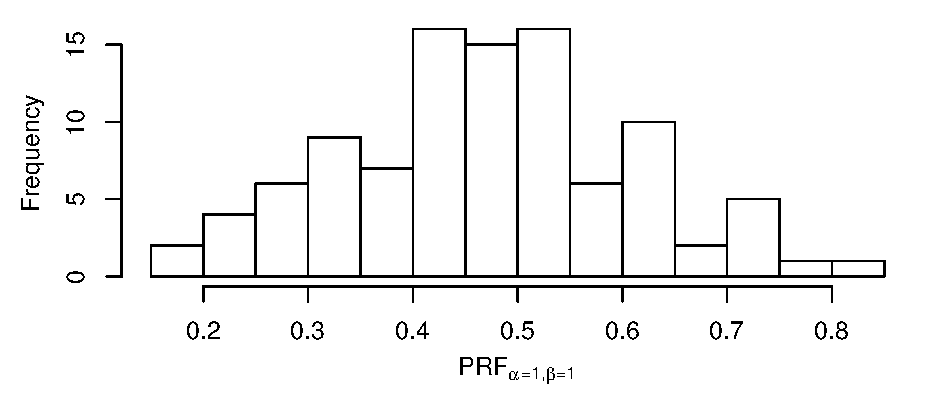
\includegraphics[width=0.8\columnwidth]{figure/qf13-qp-prf.eps}
\end{figure}

\subsection{Selective Query Faceting}
Similar to the idea of selective query expansion~\cite{cronen2004framework,amati2004query,yom2005learning} we can selectively present facets to users based on the query facet extraction performance of each query. Ideally, we only show facets for good performing queries and avoid bad ones to improve user satisfaction: in the precision-oriented scenario, it may be more desirable to leave users with a clean keyword-search interface than to show poor-quality facets. To support this selective query faceting, a key problem is the prediction of the query facet extraction performance. We find a simple score based on the expectation of \PRF can predict extraction performance fairly well.

\subsection{Performance Prediction}
In performance prediction, our goal is to predict the extraction performance for a given query with its extracted facets. We focus on predicting \PRF, and leave prediction of other measures as future work. The prediction could be done by using single indicator scores (like the clarity score in prediction retrieval performance~\cite{cronen2002predicting}), or by combining different features using regression or classification models. No matter which approach, we first need to find good indicators/features for estimating the performance. 

To find effective features, a natural way is to investigate the probabilistic model we have already learned in the QF method, because the learned probabilities already incorporate beliefs about the correctness of corresponding outputs. For example, we can use the term probability $P(y_i|t_i)$ defined in Equation~\ref{eq:y} to estimates the chance that the output terms are indeed facet terms, and use the pairs probability $P(z_{i,j}|p_{i,j},y_i,y_j)$ defined in Equation~\ref{eq:z} to estimate the chance that the term pairs in the same extracted facets indeed belong to a query facet. 

In order to use the term and pair probabilities as features, we need to aggregate them in some ways, because these probabilities are for terms and pairs, not directly for whole extracted facet set. We investigates two ways of aggregation. First, from the perspective of data fitness, we can directly use log-likelihood of extracted facets to measure the fitness. For example, we can use the whole log-likelihood based on Equation~\ref{eq:ll}, and we can also use the log-likelihood for only the terms or only the pairs based on the first term and second terms in the equation respectively. 

Second, from the perspective of directly estimating utility (performance), we can aggregate the probabilities for estimating \PRF directly in a similar way as our empirical utility maximization approach. More specially, we can estimate \PRF performance based on the expected term and pair quantities under the learned model. The estimates can be obtained as follows,
\begin{equation}
\label{eq:mest} % measure estimates
\begin{split}
\widehat{T\!P}=\frac{\sum_i P(t_i)y_i}{\sum_i y_i}, &\;\; \widehat{T\!R}=\frac{\sum_i P(t_i)y_i}{\sum_i P(t_i)},\\ 
\widehat{P\!T}=\frac{\sum_{i,j} P(p_{i,j})z_{i,j}}{\sum_{i,j} z_{i,j}},&\;\; \widehat{P\!R}=\frac{\sum_{i,j} P(p_{i,j})z_{i,j}}{\sum_{i,j} P(p_{i,j})y_iy_j},
\end{split}
\end{equation}
where we use $P(t_i)\equiv P(y_i\!=\!1|t_i)$, $P(p_{i,j})\equiv P(z_{i,j}\!=\!1|p_{i,j}, y_i\!=\!1,y_j\!=\!1)$ for simplification. Estimates of \TF, \PF and can be easily obtained by substituting \TP, \TR, \PP, \PR with their estimates in the corresponding equations in Section~\ref{sec:precision-measure}. Estimate of \PRF can be obtained by substituting \TP, \TR and \PF with their estimates in Equation~\ref{eq:prf}. We call this estimate of \PRF the ``PRF score''.

To investigate the effectiveness of the two types of features, we analyze the correlation between extraction performance and each individual feature. We show the correlation results for \QFI's \PRFab{1}{1} performance in Table~\ref{tab:cor}. (\QFI is tested using cross-validation on the \DQF dataset, which will be described in Section~\ref{sec:precision-experiment}, under maximum likelihood estimation training. Observations are similar for other runs.) 

\todo{May be I should call them posteriors}
In the table, the utility-based features \TP, \TR, \PP, \PR, \TF, \PF, $P\!R\!F\!$ (PRF score)  are estimated according to Equation~\ref{eq:mest} as described before. Likelihood-based feature $LL_{sum}=\sum_i{\log P(y_i|t_i)} + \sum_{i,j}{\log P(z_{i,j}|p_{i,j},y_i,y_j)}$ calculates the likelihood of extracted facets based on Equation~\ref{eq:ll}. $tLL_{sum}$ and $pLL_{sum}$ separate log-likelihood that accounts for term and pair in $LL_{sum}$. Average log-likelihoods $tLL_{avg}$, $pLL_{avg}$ are calculated by averaging $tLL_{sum}$ and $pLL_{sum}$ by the number of candidate terms $tSize$ and the number of pairs of selected terms (\ie, $y_i=1$), $pSize$.
\begin{table}[!ht]
\centering
\caption{The correlation of the individual features with \QFI's \PRFab{1}{1} performance. \QFI is tested using cross-validation on \DQF dataset under maximum likelihood estimation training. Feature name abbreviation explanation:  initial ``$t$'' -- ``term'', initial ``$p$'' -- ``pair'', $LL$ -- ``log-likelihood'', $avg$ -- ``average'', ``$std$'' -- ``standard deviation'', $tSize$ -- $|T_\mathcal{L}|$, $pSize$ -- $|P_\mathcal{F}|$.}
\label{tab:cor}
\begin{tabular}{|l|r|l|} \hline
Feature & Correlation & P-value\\ \hline
$P\!R\!F$ & 0.6249 & $3.6\times10^{-12}$\\ \hline
\TF & 0.5933 & $7.7\times10^{11}$\\ \hline
\TR & 0.5817 & $2.2\times10^{-10}$\\ \hline
$tLL_{avg}$ & 0.5709 & $5.5\times10^{-10}$\\ \hline
$tProb_{sum}$ & 0.5527 & $2.4\times10^{-9}$\\ \hline
$tSize$ & 0.5512 & $2.8\times10^{-9}$\\ \hline
\PF & 0.4962 & $1.5\times10^{-7}$\\ \hline
\PR & 0.4878 & $2.6\times10^{-7}$\\ \hline
%pInterProbSum & 0.4598 & $1.4\times10^{-6}$\\ \hline
$pLL_{sum}$ & -0.4513 & $2.4\times10^{-6}$\\ \hline
$pSize$ & 0.4487 & $2.8\times10^{-6}$\\ \hline
$pProb_{sum}$ & 0.4435 & $3.8\times10^{-6}$\\ \hline
%pInterSize & 0.4419 & $4.1\times10^{-6}$\\ \hline
$LL_{sum}$ & -0.4371 & $5.4\times10^{-6}$\\ \hline
\PP & 0.4015 & $3.4\times10^{-5}$\\ \hline
%$pProb_{max}$ & 0.3904 & $5.9\times10^{-5}$\\ \hline
\TP & 0.3336 & $6.9\times10^{-4}$\\ \hline
$pLL_{avg}$ & 0.3329 & $7.1\times10^{-4}$\\ \hline
%pInterProbAvg & -0.3234 & 0.0010\\ \hline
%pInterProbMin & -0.3218 & 0.0011\\ \hline
$pProb_{std}$ & -0.3162 & 0.0014\\ \hline
$tLL_{sum}$ & -0.2317 & 0.0203\\ \hline
$pProb_{min}$ & -0.1984 & 0.0478\\ \hline
$tProb_{min}$ & -0.1391 & 0.1674\\ \hline
%pInterProbMax & 0.1102 & 0.2752\\ \hline
$tProb_{std}$ & -0.1094 & 0.2787\\ \hline
$tProb_{max}$ & 0.03447 & 0.7335\\ \hline
%pInterProbStd & 0.0026 & 0.9793\\ \hline
\end{tabular}
\end{table}

From Table~\ref{tab:cor}, first we find that PRF score has strong correlation (0.6249 with p-value $3.6\times 10^{-12}$) with the performance $P\!R\!F_{\alpha=1,\beta=1}$. This suggests 1) the PRF score is a good indicator for extraction performance, and might be effective in performance prediction, and 2) our estimation of $P\!R\!F_{\alpha=1,\beta=1}$ based on its expectation is effective. Second, we find utility-based features PRF scores, $\widehat{TF}$, $\widehat{TR}$ correlate better with \PRF performance than other likelihood-based features. This validates our assumption that likelihood can be loosely related to the performance measure, and utility could be a better optimization objective.

We combine the proposed features in linear regression and logistic regression models. However, we find the results are not significantly better than simply using PRF score for prediction, which could be caused by the linear dependence between those features. Thus, we propose to use only the  PRF score for query facet extraction performance prediction, which is simple and effective as we will show in Section~\ref{sec:precision-experiment}. We also test other features based on statistical aggregates of the term and pair probabilities, including minimum, maximum, mean, sum and standard deviation. However, they show relatively low correlation with \PRF, and thus we do not report the results here. 

After choosing PRF score as the performance predictor, selective query faceting can be easily done by thresholding this score to decide to show or avoid showing query facet results for each query. We carry out experiments to evaluate its effectiveness in next.


\section{Experiments}
\label{sec:precision-experiment}
Our experiments aim to investigate mainly three research questions. First, we want to test whether existing query facet extraction methods adapt to precision-oriented scenarios. Second, we want to test if our empirical utility maximization approach is effective in precision-oriented scenarios. Last, we want to test whether the PRF score can effectively predict extraction performance, and support selective query faceting. We will first describe our experimental settings, then present experimental results for each of the research questions.

\subsection{Experimental Settings}
\subsubsection{Data}
\todo{name the data set in query face extraction chapter}
We use the same data set as in Chapter~\ref{ch:intrinsiceval}. We call the data set \DQF. \DQF contains 100 web search queries, their top 100 web search results from a commercial web search engine, and their query facet annotation. The query facet annotation was done by pooling facet results from different models, and then having the pooled terms re-grouped by human annotators into query facets. Our candidate lists are extracted as described in Chapter~\ref{ch:facet}.

\subsubsection{Evaluation}
We use \PRF as the evaluation measures, as well as term precision (\ie, \TP), term recall (\ie, \TR), and term clustering F1 (\ie, \PF). 
We choose this measure because it has the flexibility of adjusting emphasis between ``facet precision'' and ``facet recall'', which naturally suits well with the precision-oriented problem.
When $\alpha\!=\!\beta=\!1\!$, \PRFab{1}{1} is used to evaluate the case where term precision, term recall and term clustering are equally important. To evaluate facets under precision-oriented scenarios, we set a high $\alpha \in \{2, 3, \dots, 10\}$ with fixed $\beta\!=\!1$. The settings correspond to the cases where term precision is twice to ten times as important as both term recall and term clustering. Without any prior knowledge, it is more fair to assume that term precision and clustering are equally important (they are both ``precision'' factors for query facets), therefore we will focus more on only down-weighting term recall by setting $\beta \in \{\frac{1}{2}, \frac{1}{3}, ..., \frac{1}{10}\}$ or equivalently $\frac{1}{\beta} \in \{2, 3, \dots, 10\}$ with fixed $\alpha\!=\!1$. These settings correspond to the case where term precision and clustering are twice to ten times as importance as term recall. As before, we evaluate top the 10 facets returned from each model.

We use 10-fold cross validation on \DQF for training, tuning (if applicable) and testing models. Models are tuned on the same \PRF measure that they are tested on. Unless otherwise specified, statistical significance testing is performed by using paired t-test with 0.05 as the p-value threshold.

%\cmt{We will describe how we evaluate for extraction performance prediction and the selective method in Section X}

\subsubsection{Methods}
We study five query facet extraction models briefly summarized as below.
\begin{itemize}
\item \PLSA and \LDA (Section~\ref{sec:facet-other}): pLSA and LDA are applied on candidate facets for facet refining. %The assumption is like documents in the conventional setting, candidate facets are generated by a mixture of hidden topics, which are the query facets in our case. 
After training, the topics are returned as query facets, by using the top terms in each topic. We tune the number of facets and number of facet terms in each facet. The topic model methods in facet refining only uses term co-occurrence information.
\item \QDM (Section~\ref{sec:facet-other}): this is an unsupervised clustering method that applies a variation of the Quality Threshold clustering algorithm~\cite{heyer1999exploring} to cluster the candidate facets with bias towards important ones. 
%Then it ranks/selects the clusters and the terms in those clusters based on TF/IDF-like scores. 
This method incorporates more information than just term co-occurrence, but it is not easy to add new features into the model to further improve the performance.
We tune the diameter threshold, weight threshold for valid cluster and the threshold for selecting terms.
\item \QFI and \QFJ (Section~\ref{sec:facet-infer}): the two models incorporate a rich set of features and learn from labeled data. They were found to be the best across several evaluation measures in Chapter~\ref{ch:intrinsiceval}, therefore we primarily focus on them. Beyond the difference of independent and joint inference, the two models are different in that \QFI has parameters that can be tuned for given measures, while \QFJ does not, as it tries to optimize log-likelihoods. For \QFI, we tune the weight threshold for facet terms $w_{min}$, and the diameter threshold $dia_{max}$.
\end{itemize}

%In the original work, some features are extracted from candidate facets, which are extracted based on different patterns. Since the quality of the extraction patterns may vary, we expand these features by extract them from each individual types of candidate facets. This is more effective according to our experiment (, but due to space limitation, we do not report this result.) 
%supervised methods based on a graphical model, proposed in our previous work~\cite{kong2013extracting}. The graphical model learns how likely it is that a term in the candidate facets should be selected in the query facets, and how likely two terms are to be grouped together into a same query facet, using a rich set of features. Then, based on the likelihood scores, QF-I selects the terms and clusters the selected terms into query facets, while QF-J repeats the procedure, trying to performance joint inference. The two methods were shown to be more effective than the other  methods, because they incorporate more information into the models and learn from available human labels.

We study two ways of training the graphical model (see Section~\ref{sec:facet-gm}) for \QFI and \QFJ.
\begin{itemize}
\item \MLE (Section~\ref{sec:facet-train}): Uses conditional likelihood as the optimization objective and performs maximum likelihood estimating for training.
\item \EUM (Section~\ref{sec:precision-eum}): since likelihood is loosely related to the performance measure, we propose to use empirical utility maximization to directly optimize the \PRF measure during training. We approximate \PRF by its expectation in order to enable numerical optimization. With different $\alpha,\beta$, we can use different versions of \PRF as the optimization objective. We test three runs by setting $(\alpha\!=\!1,\beta\!=\!1)$, $(\alpha\!=\!2,\beta\!=\!1)$, $(\alpha\!=\!1,\beta\!=\!\frac{1}{2})$. 
%\cmt{explain why not others}. 
We denote the different runs by add $\alpha,\beta$ subscript in ``\EUM'' (\eg, \EUMab{2}{1} stands for EUM training using \PRFab{2}{1} as the optimization objective).
\end{itemize}
\subsection{Existing Methods Under Precision-Oriented Scenarios}
\label{sec:precision-existing}
We first investigate if the five existing models can adapt to precision-oriented scenarios by evaluation based on \PRF with different $\alpha,\beta$ settings. In Figure~\ref{fig:existing}, we show \PRF performance of different $\alpha$ (\ie, term precision is more important than term recall and clustering) on the left, and of different $\beta$ (\ie, term precision and clustering are more important than term recall) on the right. We test all the five models with \QFI, \QFJ trained by \MLE. 
%We report results on \DFWS (observations are similar for \DQF).
\begin{figure}[!ht]
\centering
\caption{$P\!R\!F_{\alpha,\beta}$ performance with different $\alpha$ (left, fixed $\beta\!=\!1$) and different $\beta$ (fixed $\alpha\!=\!1$, right) settings for existing methods on \DQF.}
\label{fig:existing}
\begin{subfigure}[b]{0.45\columnwidth}
\includegraphics[width=\columnwidth]{figure/qf13-prfa-5models.eps}
\caption{\DQF, $P\!R\!F_{\alpha,\beta=1}$}
\end{subfigure}
\begin{subfigure}[b]{0.45\columnwidth}
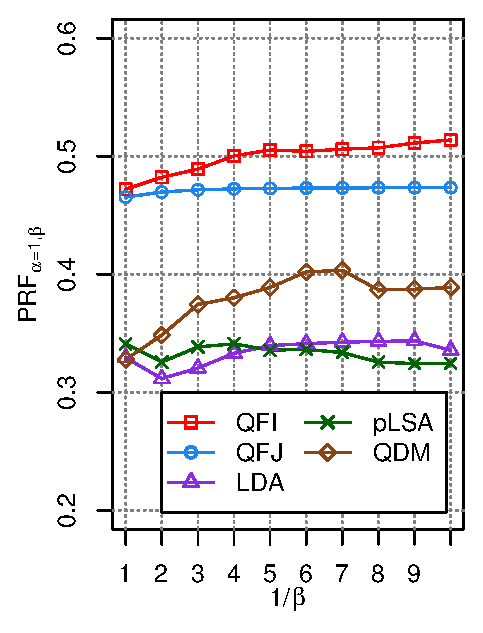
\includegraphics[width=\columnwidth]{figure/qf13-prfaf-5models.eps}
\caption{\DQF, $P\!R\!F_{\alpha=1,\beta}$}
\end{subfigure}
%\begin{subfigure}[b]{0.49\columnwidth}
%\includegraphics[width=\columnwidth]{fws14-prfa-5models}
%\caption{$P\!R\!F_{\alpha,\beta=1}$}
%\end{subfigure}
%\begin{subfigure}[b]{0.49\columnwidth}
%\includegraphics[width=\columnwidth]{fws14-prfaf-5models}
%\caption{$P\!R\!F_{\alpha=1,\beta}$}
%\end{subfigure}
\end{figure}

%First, from Figure~\ref{fig:existing}, we can see pLSA and LDA are generally less effective comparing to other models in both the normal case (\ie, \PRFab{1}{1}) and precision-oriented cases. This suggests topic modeling approach, which only incorporates term co-occurrence information, does not suit the facet extraction problem well, which was also find in the previous work~\cite{kong2013extracting}.
First, we find \QFJ does not adapt well to precision-oriented scenarios. From the figure, we can see the superiority of \QFJ over other models becomes less evident, when moving from the normal case (low $\alpha$ or high $\beta$) to precision-oriented cases (high $\alpha$ or low $\beta$). This because that \QFJ tries to optimize log-likelihood for inferencing, and it cannot be tuned on the performance measures like other models. So it returns the same results for the normal case and precision-oriented scenarios. Second, we generally find that \QFI and \QDM can adapt better than the other models to the precision-oriented scenarios, with \QFI consistently better than all the other models on both datasets. The adaptability of the two models can be explained by their tuning procedure. For example, depending on the target performance measure, \QFI can set different threshold $w_t$ for selecting facet terms. Overall, we find \QFI (under \MLE training) is the best among these existing models for the normal case, as 
well as precision-oriented cases.
 
To further analyze how \QFI adapts to the precision-oriented scenarios, in Table~\ref{tab:qfi}, we report \PRF together with \TP, \TR, \PF and facet size (the total number of terms returned for a query) when setting different $\beta$ in \PRF. 
%For comparison, we also include the results of \QFJ in the last row. Please note \QFJ's \TP, \TR, \PF are all the same for all $\beta$ settings (\ie, no tuning capability), and its \PRF performance is based $\alpha\!=\!1,\beta\!=\!1/10$. 
\begin{table}[!ht]
\centering
\caption{$P\!R\!F_{\alpha,\beta}$ performance with its \TP, \TR, \PF under different $\beta$ settings (fixed $\alpha\!=\!1$) for \QFI on \DQF. ``Size'' reports the average number of terms returned for each queries.}
\label{tab:qfi} 
\begin{tabular}{|r|l|l|l|l|l|} \hline
$\frac{1}{\beta}$ & \PRF & TP & TR & PF & Size\\ \hline
1 & 0.4720 & 0.4450 & 0.4881 & 0.6209 & 89.5\\ \hline
2 & 0.4822 & 0.4896 & 0.4186 & 0.6192 & 70.7\\ \hline
3 & 0.4891 & 0.5108 & 0.3574 & 0.5989 & 56.5\\ \hline
4 & 0.5003 & 0.5291 & 0.3498 & 0.5925 & 53.0\\ \hline
5 & 0.5053 & 0.5348 & 0.3306 & 0.5928 & 48.9\\ \hline
6 & 0.5042 & 0.5343 & 0.3194 & 0.5834 & 47.1\\ \hline
7 & 0.5060 & 0.5343 & 0.3194 & 0.5834 & 47.1\\ \hline
8 & 0.5072 & 0.5343 & 0.3194 & 0.5834 & 47.1\\ \hline
9 & 0.5112 & 0.5364 & 0.3172 & 0.5864 & 46.7\\ \hline
10 & 0.5138 & 0.5365 & 0.3097 & 0.5824 & 45.2\\ \hline
%\hline QFJ & 0.4734 & 0.3986 & 0.4832 & 0.6961 & 97.0\\ \hline
\end{tabular}
\end{table}

From Table~\ref{tab:qfi}, we find that as term recall factor becomes less and less important (or equivalently as the precision factors becomes more and more important), \QFI becomes more and more conservative in selecting terms. The number of terms returned on average for each query (``size'' in the table) decreases from 89.5 to 45.2. Term precision \TP thus increases significantly, while term recall \TR and term clustering \PF decrease. This indicates, by tuning on the performance measure, \QFI tries to find a good balance between the tree factors for each scenarios. 

\subsection{Empirical Utility Maximization Performance}
Next, we compare \EUM  and \MLE training to test the effectiveness of the EUM approach we proposed. We first compare \EUM and \MLE training using both \QFI and \QFJ in Figure~\ref{fig:ll-prf}. We report results for $P\!R\!F_{\alpha=1,\beta}$ (\ie, fixed $\alpha=1$ with different $\beta$ settings) on \DQF. Observations are similar for other cases. The figure shows \QFI with \EUM and \MLE training on the left, and \QFJ results on the right. We report three runs of \EUM, which use \PRF under different $\alpha,\beta$  settings (specified in the legend) as the training target.


\begin{figure}[!ht]
\centering
\caption{$P\!R\!F_{\alpha=1,\beta}$ performance for \MLE and \EUM training using \QFI (left) and \QFJ (right) on \DQF. The three \EUM runs use \PRF under different $\alpha,\beta$ settings (specified in the legend) as the training target.}
\label{fig:ll-prf}
\begin{subfigure}[b]{0.45\columnwidth}
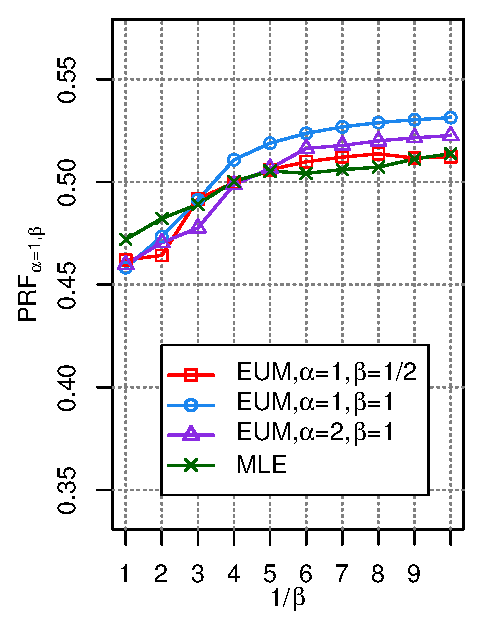
\includegraphics[width=\columnwidth]{figure/qf13-qfi-prfaf-ll-prf.eps}
\caption{\QFI}
\end{subfigure}
\begin{subfigure}[b]{0.45\columnwidth}
\includegraphics[width=\columnwidth]{figure/qf13-qfj-prfaf-ll-prf.eps}
\caption{\QFJ}
\end{subfigure}
%\begin{subfigure}[b]{0.49\columnwidth}
%\includegraphics[width=\columnwidth]{figure/fws14-qfi-prfaf-ll-prf.eps}
%\caption{\DFWS, \QFI}
%\end{subfigure}
%\begin{subfigure}[b]{0.49\columnwidth}
%\includegraphics[width=\columnwidth]{figure/fws14-qfj-prfaf-ll-prf.eps}
%\caption{\DFWS, \QFJ}
%\end{subfigure}
\end{figure}

From Figure~\ref{fig:ll-prf}, for \QFI, we find there are no statistically significant differences between \MLE and \EUM in most cases, even though generally \EUM obtains slightly better \PRF than \MLE. This can be explained by noting that \QFI under \MLE has already incorporated the \PRF learning target because it is tuned on \PRF. Essentially, we can view \QFI (under \MLE training) as a model that is trained on likelihood to find a small tuning space to enable optimization on given performance measures by hand tuning.

Differently, for \QFJ, we find \EUM can improve largely over \MLE under the precision-oriented scenarios. The differences between \EUM and \MLE are statistically significant for all $1/\beta>2$ and for all the three \EUM runs. This indicates 1) utility (performance measure) is a better optimization objective than likelihood and 2) our approximation of \PRF based on its expectation is effective. 


To study how \EUM training affects \QFJ in more details, as an example, we show \PRFab{1}{0.1} together with its \TP, \TR, \PF and facet size in Table~\ref{tab:prf}.
\begin{table}[!ht]
\centering
\caption{\PRFab{1}{0.1} with \TP, \TR, \PF for \MLE and \EUM training on \DQF. Subscripts of \EUM indicates the $\alpha,\beta$ setting used for its optimization target \PRF. }
\label{tab:prf}
\begin{tabular}{|l|l|l|l|l|l|l|} \hline
model & Training & \PRF & TP & TR & PF & Size\\ \hline
%\QFI & \MLE & 0.5138 & 0.5365 & 0.3097 & 0.5824 & 45.2\\ \hline
%\QFI & \EUMab{1}{1} & 0.5123 & 0.5250 & 0.2999 & 0.6021 & 45.7\\ \hline
%\QFI & \EUMab{2}{1} & 0.5226 & 0.5455 & 0.2588 & 0.6073 & 37.8\\ \hline
%\QFI & \EUMab{1}{0.5} & 0.5313 & 0.5426 & 0.2724 & 0.6180 & 41.0\\ \hline\hline
\QFJ & \MLE & 0.4734 & 0.3986 & 0.4832 & 0.6961 & 97.0\\ \hline
\QFJ & \EUMab{1}{1} & 0.5223 & 0.4884 & 0.3341 & 0.6702 & 54.8\\ \hline
\QFJ & \EUMab{2}{1} & 0.5696 & 0.5711 & 0.2328 & 0.6705 & 33.9\\ \hline
\QFJ & \EUMab{1}{0.5} & 0.5607 & 0.5710 & 0.2229 & 0.6620 & 33.0\\ \hline
\end{tabular}
\end{table}

From Table~\ref{tab:prf}, first, we can see when trained on \EUM under precision-oriented settings (\ie,\EUMab{2}{1} and \EUMab{1}{0.5}), \QFJ are more conservative in selecting terms than in \MLE training. When moving from \MLE to \EUM training, its facet size becomes much smaller (\ie, 97 to 33), \TP increases greatly while \TR decreases substantially. This effect is desirable under the precision-oriented scenarios, in which we care much more about precision than recall, as reflected by the improvement in \PRFab{1}{0.1} shown in the table.

Second, by comparing \EUMab{1}{1} with \EUMab{2}{1}, \EUMab{1}{0.5} in Table~\ref{tab:prf}, we can see \EUMab{2}{1}, \EUMab{1}{0.5} trained models behave more conservatively than \EUMab{1}{1} trained models. This suggest our training is effective -- as we change the training target \PRF parameter from $(\alpha=1,\beta=1)$ to $(\alpha=2,\beta=1)$ and $(\alpha=1,\beta=0.5)$), it learns that we are putting more emphasis on precision, and thus behaves more conservatively.

Last, the improvement of \QFJ in precision oriented scenarios raises a question -- will it outperform the previous best model, \QFI, under precision-oriented scenarios? We test this in Figure~\ref{fig:qfi-qfj}. In the figure, we compare \QFJ under \EUM training with other baselines, including \QFI under \MLE (representing the state-of-the-art baseline) and \EUM training. We report results under \EUMab{1}{0.5} training on \DQF (results are similar in other cases). From the figure we find \QFJ under \EUM training outperforms other models in the precision-oriented scenarios. The difference between \QFJ,\EUM and the state-of-the-art method \QFI,\MLE are statistically significant for $P\!R\!F_{\alpha=1,\beta}$ when $\frac{1}{\beta}>4$.
\begin{figure}[!ht]
\centering
\caption{\PRF performance with different $\alpha$, $\beta$ settings for \QFI and \QFJ under \MLE and \EUM training on \DQF. \EUMab{1}{0.5} run result is reported for \EUM.}
\label{fig:qfi-qfj}
\begin{subfigure}[b]{0.45\columnwidth}
\includegraphics[width=\columnwidth]{figure/qf13-prfa-qfi-qfj.eps}
\caption{$P\!R\!F_{\alpha,\beta=1}$}
\end{subfigure}
\begin{subfigure}[b]{0.45\columnwidth}
\includegraphics[width=\columnwidth]{figure/qf13-prfaf-qfi-qfj.eps}
\caption{$P\!R\!F_{\alpha=1,\beta}$}
\end{subfigure}
%\begin{subfigure}[b]{0.49\columnwidth}
%\includegraphics[width=\columnwidth]{fws14-prfa-qfi-qfj}
%\caption{\DFWS, $P\!R\!F_{\alpha,\beta=1}$}
%\end{subfigure}
%\begin{subfigure}[b]{0.49\columnwidth}
%\includegraphics[width=\columnwidth]{fws14-prfaf-qfi-qfj}
%\caption{Fws14, $P\!R\!F_{\alpha,\beta=1}$}
%\end{subfigure}
\end{figure}

\subsection{Extraction Performance Prediction}
To predict query facet extraction performance, we build linear regression models using only the PRF score (see Section~\ref{sec:precision-selective}) as the feature (with intercept). We test the models for predicting \PRF under different $\alpha,\beta$, based on 10-fold cross validation on \DQF for \QFI in Table~\ref{tab:regression}. We report root-mean-square deviation (RMSD), Pearson correlation (R), and p-values for the significance of correlation. %(observations are similar for \QFJ runs). 
\begin{table}[!ht]
\centering
\caption{Linear regression results based on 10-fold cross-validation for predicting \PRF performance. RMSD -- root-mean-square deviation, R -- Pearson correlation.}
\label{tab:regression}
\begin{tabular}{|l|l|l|l|} \hline
Measure & RMSD & R & p-value\\ \hline
\PRFab{1}{1} & 0.1110 & 0.6112 & $1.4\times10^{-11}$\\ \hline
\PRFab{1}{0.2} & 0.1800 & 0.5745 & $4.1\times 10^{-10}$\\ \hline
\PRFab{1}{0.1} & 0.1882 & 0.5566 & $1.8\times 10^{-9}$\\ \hline
\PRFab{5}{1} & 0.2109 & 0.2958 & 0.0028\\ \hline
\PRFab{10}{1} & 0.2245 & 0.4028 & $3.2\times 10^{-5}$\\ \hline
%\hline
%\QFJ & \PRFab{1}{1} & 0.1177 & 0.5916 & $9.1\times 10^{-11}$\\ \hline
%\QFJ & \PRFab{1}{0.2} & 0.2073 & 0.4717 & $7.2\times 10^{-7}$\\ \hline
%\QFJ & \PRFab{1}{0.1} & 0.2239 & 0.4164 & $1.6\times 10^{-5}$\\ \hline
%\QFJ & \PRFab{5}{1} & 0.2057 & 0.4189 & $1.4\times 10^{-5}$\\ \hline
%\QFJ & \PRFab{10}{1} & 0.2360 & 0.3182 & 0.0013\\ \hline
\end{tabular}
\end{table}

The results in Table~\ref{tab:regression} show fairly strong RMSD values and strong positive correlations between the predicted \PRF and real \PRF performance for most cases. For example, p-value $1.4\times10^{-11}$ for the first row indicates that it is extremely unlikely that the predicted \PRFab{1}{1} performance has no relationship with the actual performance. We also see one exception. For \PRFab{5}{1} we only see fair correlation, which may be because that we use $\alpha\!=\!1,\beta\!=\!1$ for computing our PRF score, while in \PRFab{5}{1} the three factors are more unbalanced weighted.

\subsection{Evaluating Selective Query Faceting}
Next, we study the effectiveness of selective query faceting based on the predicted score (from cross validation). Recall that our selective method is done by thresholding the predicted performance for deciding whether to show or avoid showing facets for each query (see Section~\ref{sec:precision-selective}). There is a trade-off between the performance of selected queries and the coverage of queries for query faceting. With a higher threshold, selective query faceting would select fewer queries to show facets, but users should obtain better performance for the facets that are presented to them. On the contrary, a lower threshold will result in selecting more queries to show facets, but the performance for the selected queries may be worse. 

To evaluate selective query faceting, we plot the average \PRF performance for queries selected by PRF score, when using different thresholds in Figure~\ref{fig:selective}. The x-axis indicates the number of selected queries, while the y-axis indicates the average \PRF performance for those selected queries. In addition to average \PRF, we also plot the standard error with 95\% confidence intervals by the gray area (except for the case where only one query is selected). We report results on \DQF for a \QFI run that are trained under \MLE and evaluated on \PRFab{1}{1}. 
%(Observations for other runs are similar.) 
%The two runs represent the best model for normal cases and precisely-oriented scenarios respectively.
\todo{Need to stress that the number of queries changes. So the comparison may make no sense}

\begin{figure}[!ht]
\centering
\caption{Average \PRF performance for selected queries. The gray area indicates standard error with 95\% confidence intervals. Run: \PRFab{1}{1} as the measure with \MLE trained \QFI as the extraction model}
\label{fig:selective}
\includegraphics[width=0.8\columnwidth]{figure/qf13-qp-prf-ll.eps}
%\begin{subfigure}[b]{1\columnwidth}
%\includegraphics[width=0.8\columnwidth]{qf13-qp-prf-ll}
%\end{subfigure}
%\begin{subfigure}[b]{1\columnwidth}
%\includegraphics[width=\columnwidth]{qf13-qp-prfb01-prfb05}
%\caption{Run: \PRFab{1}{0.1} as measure with \EUMab{1}{0.5} trained \QFJ extraction model.}
%\end{subfigure}
\end{figure}

From Figure~\ref{fig:selective}, we can see as we select fewer and fewer queries for presenting facets, generally the average performance for the selected queries increases. This indicates the query faceting method is fairly effective in selecting good performing queries and avoiding bad ones. When 20 queries are selected, we obtain 0.5792 \PRFab{1}{1} for the selected queries, comparing to 0.4720 when the selective method is not performed (\ie, showing facets for all queries). The difference are statistically significant according to two-tailed two-sample t-test (p-value = 0.0034). 

%The observation for Figure~\ref{fig:selective}(b) is similar but less evident. We also find statistical significant improvement when applying selective faceting. For example, when selecting 20 queries, we obtain 0.6986 \PRFab{1}{0.1}, comparing to 0.5607 when the selective method are not performed (p-value = 0.0011).

\section{Summary}
\label{sec:precision-conclusion}
In this chapter, we studied and improved query facet extraction under precision-oriented scenarios, which could help this technique to be used practically. We find the performance expectation can be used as an approximation to directly optimize the performance measure, which significantly improves existing models under precision-oriented scenarios. We proposed a PRF score based on the expectation of \PRF to predict extraction performance. We show this score has fairly good prediction performance which enables selective query faceting that selects good performing queries to show facets, and improves the average extraction performance.

In next chapter, we will consider how to re-organize search results based on users' selection on the extracted query facets.